\documentclass[a4paper, 11pt]{article}

\usepackage[left=1.5cm, right=1.5cm, top=2cm, bottom=2cm]{geometry}

\usepackage[utf8]{inputenc} 
\usepackage[T1]{fontenc}      
\usepackage[french,english]{babel}  
\usepackage{lmodern}

\usepackage{amsmath, mathtools}
\usepackage{amssymb}
\usepackage{amsthm}
\usepackage{empheq}

\usepackage{graphicx,wrapfig}
\usepackage{subfig}

\usepackage{listings}
\usepackage{color} %red, green, blue, yellow, cyan, magenta, black, white
\definecolor{mygreen}{RGB}{28,172,0} % color values Red, Green, Blue
\definecolor{mylilas}{RGB}{170,55,241}

\graphicspath{{../figures/}}
\usepackage{caption}

\begin{document}
\title{Rendu DM1 Modèles probabilistes graphiques} 
\author{Yoann Pradat}
\maketitle

\paragraph{Exercise 1}

Let $(x_i, z_i)_{i=1,\dots,n}$ be the observations with $n \in \mathbf{N}^*$ the number of observations. To compute the
MLE of the parameters $\pi$ and $\theta$ let's maximize the log of the joint likelihood on $x$ and $z$.\\

$\log p_{\theta}(x, z) = \sum_{i=1}^n \log(p_{\theta}(x_i,z_i))=\sum_{i=1}^n \log(p_{\theta}(z_i)p_{\theta}(x_i|z_i))$ \\

\smallbreak

i.e $\log p_{\theta}(x, z) =\sum_{i=1}^n \sum_{m=1}^M z_i^m \log(\pi_m) + \sum_{i=1}^n \sum_{m=1}^M \sum_{k=1}^K z_i^m
x_i^k \log(\theta_{mk})$\\ 

where $z_i^m = 1$ if $z_i = m$, 0 otherwise and same for $x_i^k$. \\

To estimate $\pi=(\pi_1, \dots, \pi_M)$ we want to solve $\max\limits_{\pi, \sum_m \pi_m = 1} \sum_{i=1}^n \sum_{m=1}^M
z_i^m \log(\pi_m)$ which is a constrained optimization. To achieve that we maximize the Lagrangian $\mathcal{L} = 
\sum_{i=1}^n \sum_{m=1}^M z_i^m \log(\pi_m) + \lambda (1-\sum_{m=1}^M \pi_m)$. \\

$\bullet$ We find the MLE estimator of $\pi_m$ to be \fbox{$\pi_m^* = \frac{\sum_{i=1}^n z_i^m}{n}$}. \\

To estimate $\theta$ we want to solve $\max\limits_{\theta, \forall m \sum_k \theta_{mk} = 1} \sum_{i=1}^n \sum_{m=1}^M 
\sum_{k=1}^K z_i^m x_i^k \log(\theta_{mk}) $ which is a constrained optimization. The associated Lagrangian $\mathcal{L} 
= \sum_{i=1}^n \sum_{m=1}^M \sum_{k=1}^K z_i^m x_i^k \log(\theta_{mk}) + \sum_{m=1}^M \lambda_m  (1-\sum_{k=1}^K
\theta_{mk})$. \\

$\bullet$ We find the MLE estimator of $\theta_{mk}$ to be \fbox{$\theta_{mk}^* = \frac{\sum_{i=1}^n z_i^m
x_i^k}{\sum_{i=1}^n \sum_{l=1}^K z_i^m x_i^l}$}. \\

\paragraph{Exercise 2}

2.1.(a) Let $(x_i, z_i)_{i=1,\dots,n}$ be the observations. The log likelihood is: \\

$\log p_{\theta}(x, y) =\sum_{i=1}^n \sum_{k=0}^1 y_i^k \log(\pi_k) - \sum_{i=1}^n \sum_{k=0}^1 y_i^k \big[ \log(2\pi)
+ \frac{1}{2} \log(\det \Sigma) + \frac{1}{2} (x_i - \mu_k)^t \Sigma^{-1} (x_i-\mu_k) \big] $\\

Maximizing separately over $\pi=\pi_1$, $\mu_k$ and $\Sigma$ we find MLEs to be \fbox{$\pi^* = \frac{\sum_{i=1}^n
y_i^1}{n}$}, \fbox{$\mu_k^* = \frac{\sum_{i=1}^n y_i^k x_i}{\sum_{i=1}^n y_i^k}$} k=0,1 and \fbox{$\Sigma^* = \frac{1}{n}
\sum_{i=1}^n \sum_{k=0}^1 y_i^k (x_i-\mu_k)(x_i-\mu_k)^t$}. \\

Using Bayes formula we can write $p(y=1|x) = \frac{p(x|y=1)p(y=1)}{p(x)}$ with $p(y=1)=\pi$ and $p(x|y=1)$ is Gaussian.
All worked out, the form is comparable to that of logistic regression $p(y=1|x) = \sigma(a+b^tx)$ with:
\begin{center} \fbox{$a = \log(\frac{\pi}{1-\pi}) + \frac{1}{2}(\mu_0^t\Sigma^{-1}\mu_0 - \mu_1^t\Sigma^{-1}\mu_1)$ and
$b=\Sigma^{-1}(\mu_1-\mu_0)$} \end{center} 

2.5.(a) The log likelihood is:\\
$\log p_{\theta}(x, y) =\sum_{i=1}^n \sum_{k=0}^1 y_i^k \log(\pi_k) - \sum_{i=1}^n \sum_{k=0}^1 y_i^k \big[ \log(2\pi)
+ \frac{1}{2} \log(\det \Sigma_k) + \frac{1}{2} (x_i - \mu_k)^t \Sigma_k^{-1} (x_i-\mu_k) \big] $

Again, we find the same MLE for $\pi$ and $\mu_k$ as in 2.1.(a). However for $\Sigma_k$ k=0,1 we find:
\begin{center} \fbox{$\Sigma_k^* = \frac{\sum_{i=1}^n y_i^k (x_i-\mu_k)(x_i-\mu_k)^t}{\sum_{i=1}^n y_i^k} $}. \end{center} 

We then show that \fbox{$p(y=1|x) = \sigma(\log(\frac{\pi}{1-\pi}) + \frac{1}{2}\log(\frac{\det \Sigma_1}{\det \Sigma_0}) +
\frac{1}{2}\big[(x-\mu_0)^t\Sigma_0^{-1}(x-\mu_0) - (x-\mu_1)^t\Sigma_1^{-1}(x-\mu_1)\big])$}.


\newpage

\begin{figure}[!h]
\centering
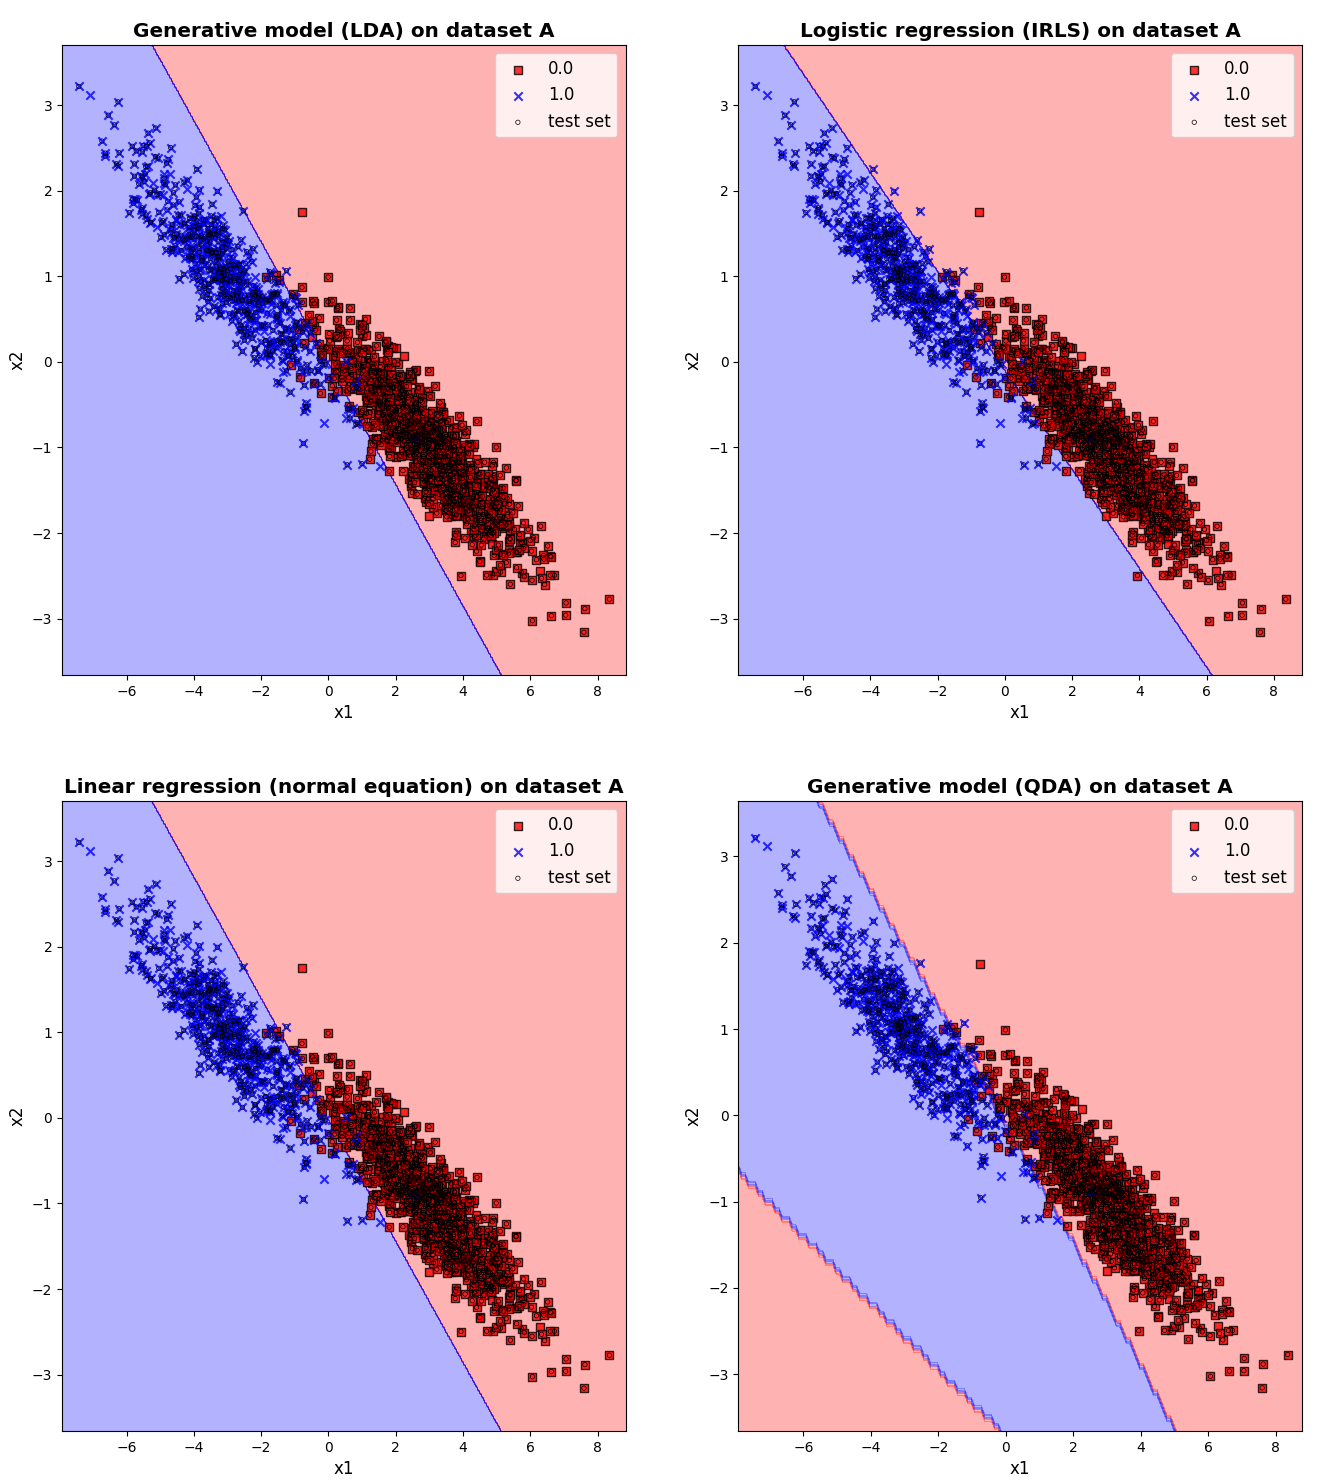
\includegraphics[width=16cm]{dataset_A_crop.png}
\caption{Boundaries representations on dataset A}
\end{figure}

\noindent\begin{minipage}[b]{0.5\linewidth}
\centering
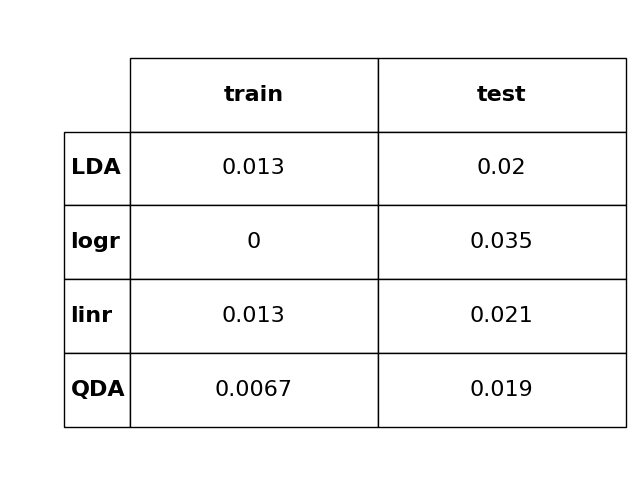
\includegraphics[width=7cm]{dataset_A_table.png}
\captionof{figure}{Misclassification errors on dataset A}
\end{minipage}%
\hfill
\begin{minipage}[b]{0.5\linewidth}
All models have misclassifications errors below 5\% on training and test set. This error is always lower on the training
set than on the test. It comes from the fact that training the model means finding the parameters that work best on the 
training data. Therefore, the model works at his best on the data on which it was optimized and we can only expect as good 
or least good average performances on the test set. \textbf{Logistic regression} outperforms all models (0\% error !) on 
the training data but underperforms all models on the test set. We said that this model presents the \textbf{largest overfit}.
\textbf{LDA} and \textbf{linear regression} have very similar results on this dataset and \textbf{QDA} seems to be the
best model.
\end{minipage}

\newpage

\begin{figure}[!h]
\centering
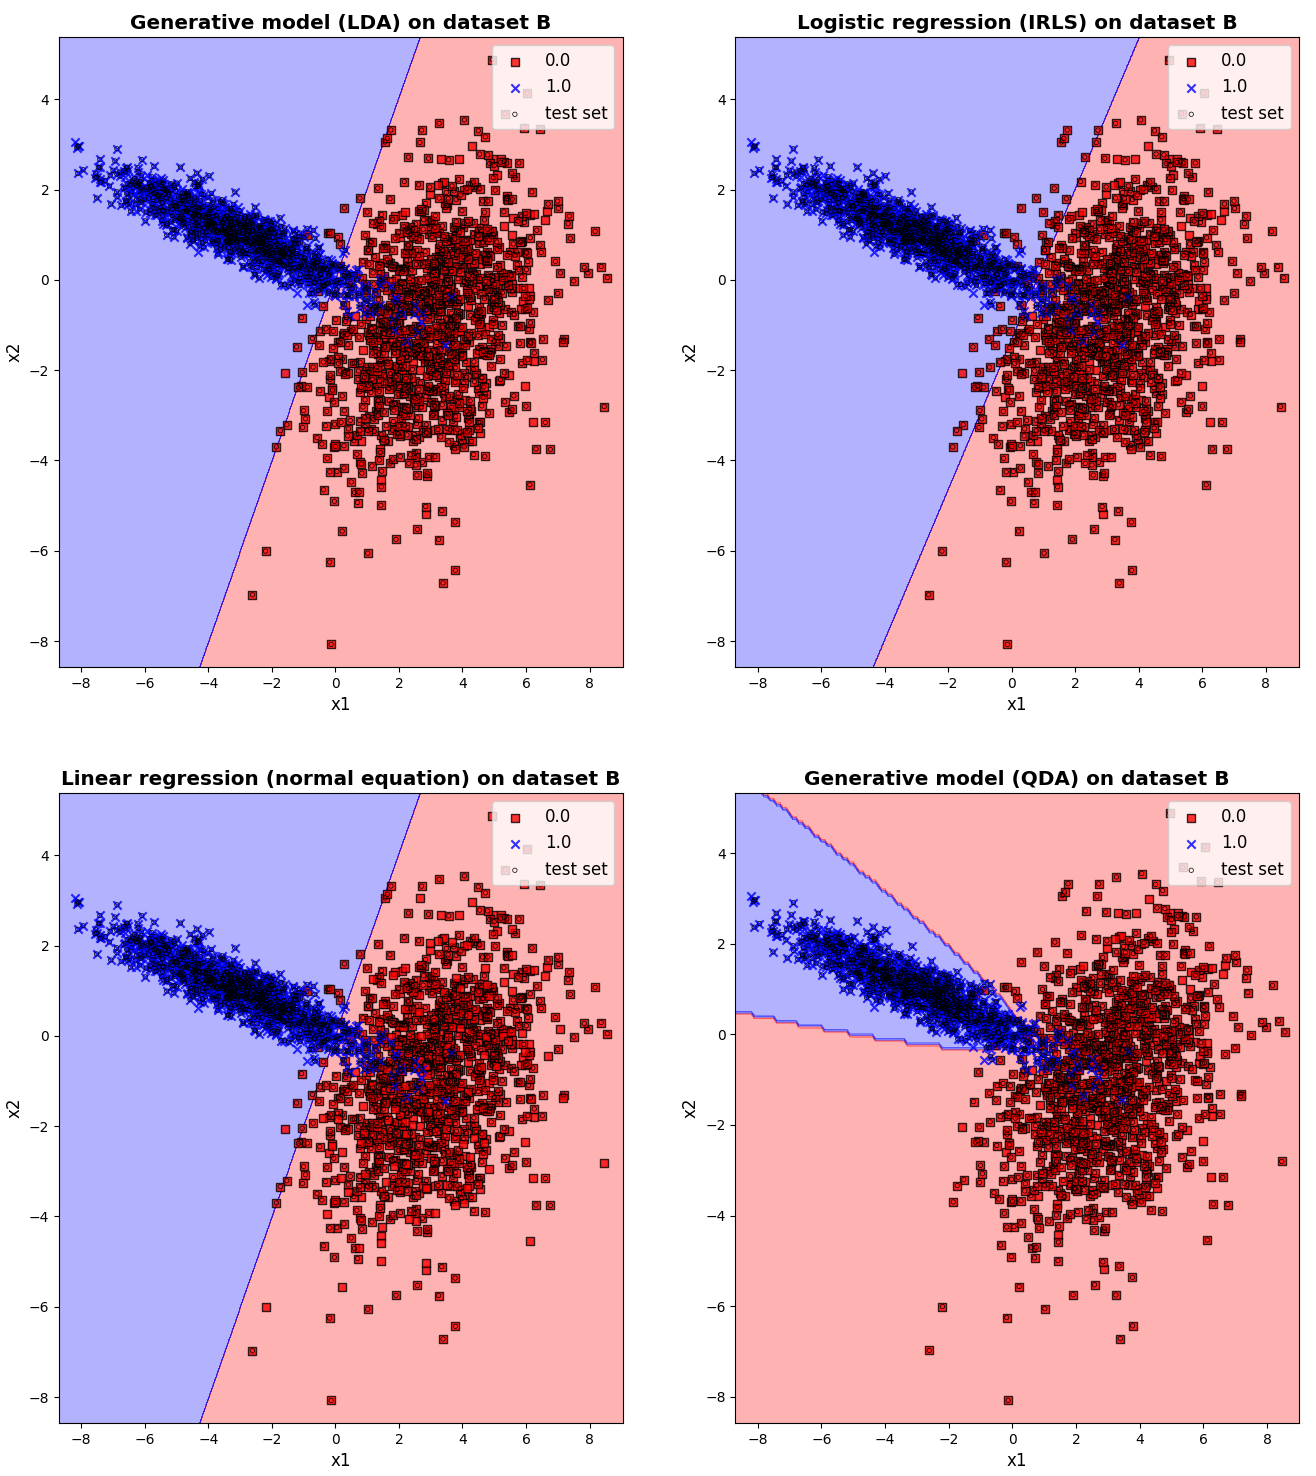
\includegraphics[width=16cm]{dataset_B_crop.png}
\caption{Boundaries representations on dataset B}
\end{figure}

\noindent\begin{minipage}[b]{0.5\linewidth}
\centering
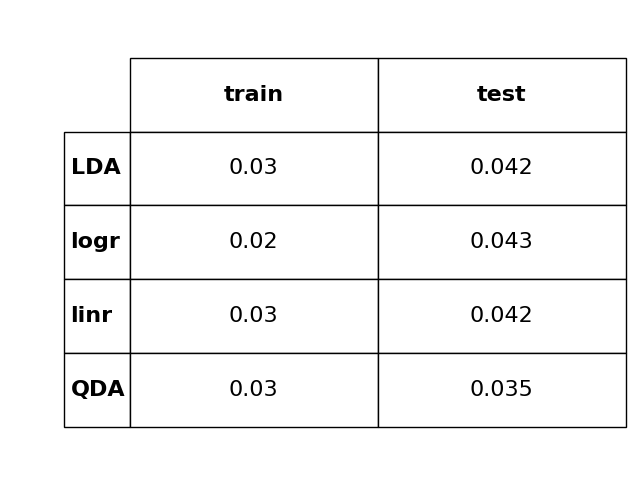
\includegraphics[width=7cm]{dataset_B_table.png}
\captionof{figure}{Misclassification errors on dataset B}
\end{minipage}%
\hfill
\begin{minipage}[b]{0.5\linewidth}
The observations in the dataset A also hold for dataset B. Logistic regression has the largest overfit, QDA is the
best model (lowest error on test set) and linear regression and LDA are identical. At first sight it seems a bit
surprising that a discriminative model (the linear regression) making assumptions on $p(y|x)$ proves to be identical to
a generative model (LDA) that models $p(x,y)$. Some research showed that this is always true when the
dependent variable consists in 2 groups though the maths behind that statement are not that obvious. QDA is slightly
better as the \textbf{assumption} $\Sigma_0 = \Sigma_1$ of LDA seems to be \textbf{incorrect} on this dataset.
\end{minipage}

\newpage

\begin{figure}[!h]
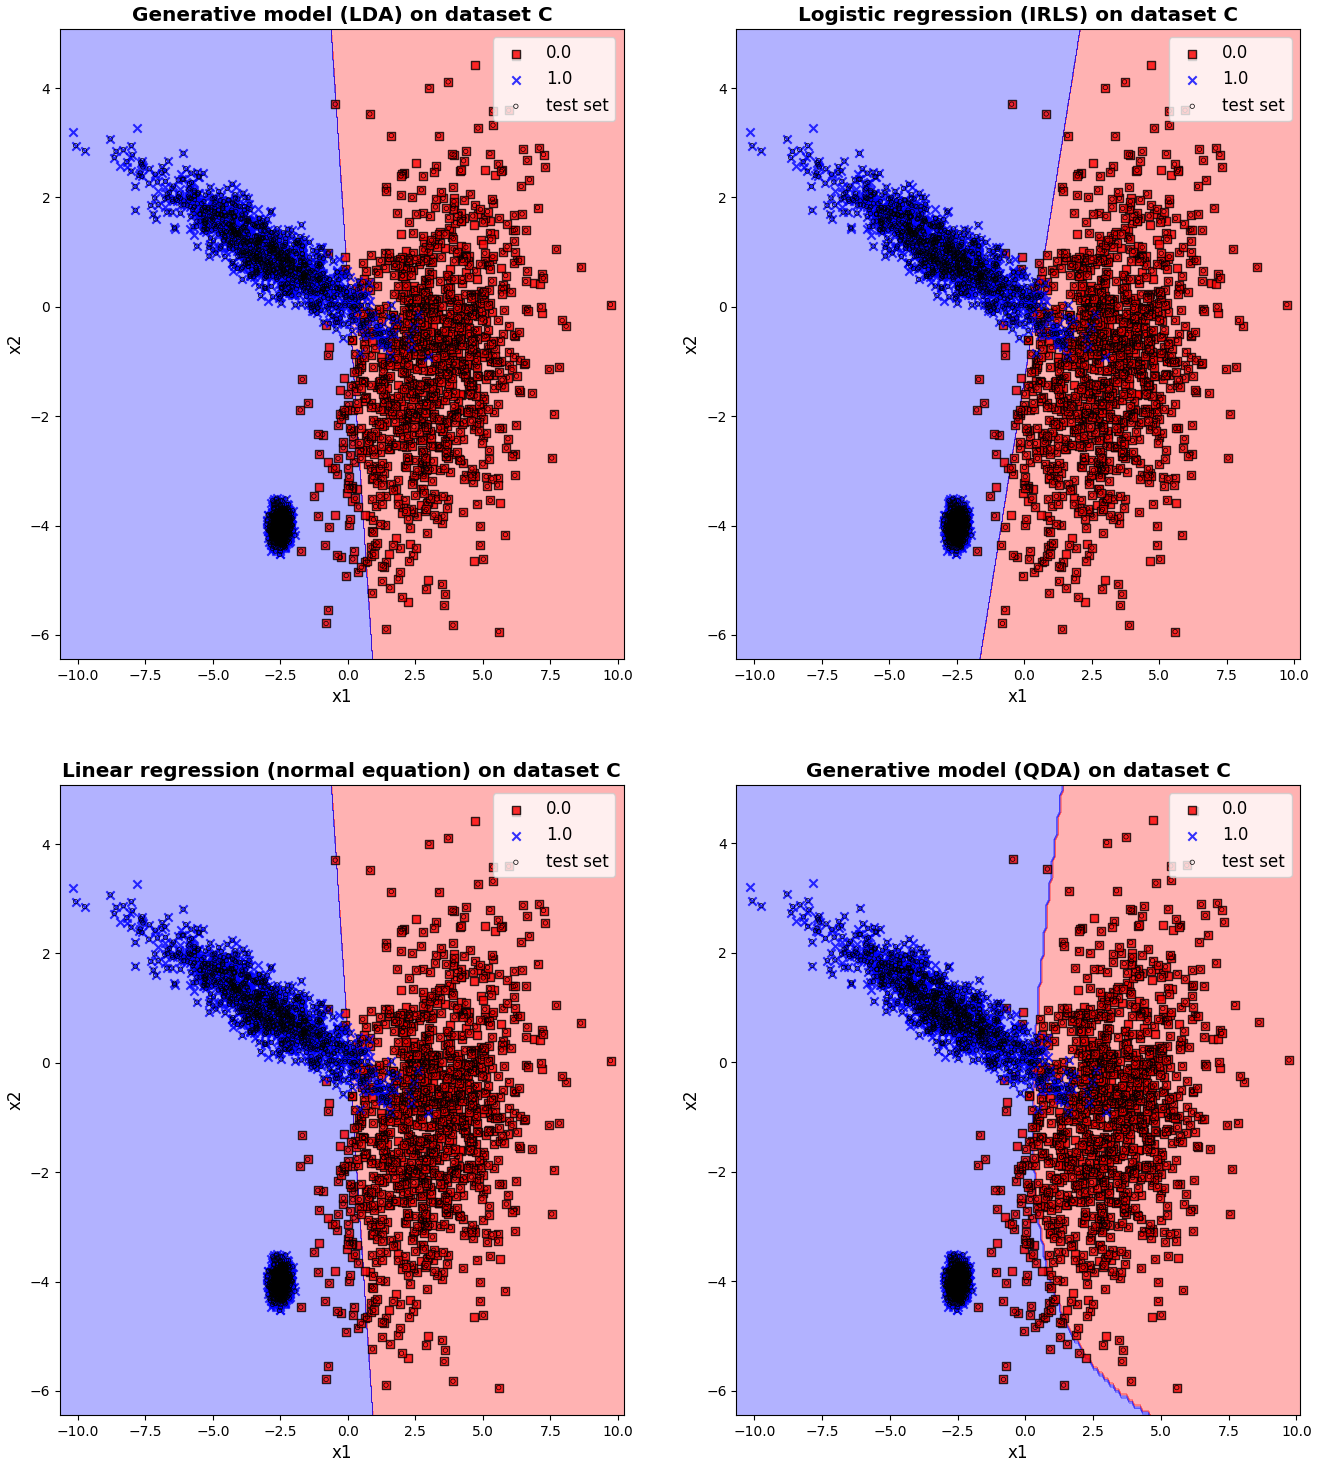
\includegraphics[width=16cm]{dataset_C_crop.png}
\caption{Boundaries representations on dataset C}
\end{figure}

\noindent\begin{minipage}[b]{0.5\linewidth}
\centering
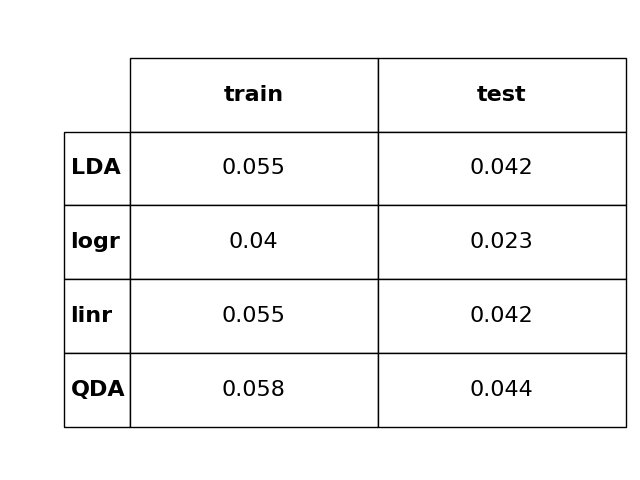
\includegraphics[width=7cm]{dataset_C_table.png}
\captionof{figure}{Misclassifications errors on dataset C}
\end{minipage}%
\hfill
\begin{minipage}[b]{0.5\linewidth}
On this dataset C, the conclusions are reversed compared to A and B. Logistic regression outperforms other models on the
test set. Given the representation above, it is quite clear that $X|Y=1$ is not normally distributed at all. It looks
more like a mixture of gaussians. Therefore the \textbf{assumptions} underlying QDA and LDA models are \textbf{grossly 
incorrect} while the assumption behind logistic regression looks more reasonable. The performances of these algorithms 
confort us in our explanations. 
\end{minipage}



\end{document}



